\cotefile{156-5}
\scanpage{26}\mspage{25}
% @ top, lines 1–4
(resp. \unsure{ouvert}, resp. loc. fer.) est idem. Le cas d'une \deleted{\unsure{sur|su|sub}}subdivision est celui où $S=T$, i.e. s'explicite comme une situation
% @ upper centre, diagram
\diagram{\begin{tikzcd}[ampersand replacement=\&,row sep=large]
 S \arrow[r,hook] \arrow[d,"p"'," {\text{surj}}"] \& \mathcal{L}\\
 I \arrow[d,"\varphi"'," {\text{surj.}}"] \& {}\\
 J \& {,}
\end{tikzcd}}
% slanted
% @ upper left, oblique note lines 1–8
\margin{Attention au cas où $\varphi$ est bijective, sans être un iso (deux structures d'ordre diff. sur un $=$ $I$, avec l'une plus fine que l'autre). C'est le cas d'un $F\unsure{\preceq|\leq}G$, avec $F\ne G$, et pourtant $=$ relation \deleted{\unsure{d'éq}} $\unsure{\mathcal R|\mathscr R}_{F}=\mathcal R_{G}$ sur $|F|=|G|$.}
% @ beneath diagram
en posant $q=\varphi\circ p$.

% @ centre, heading
\uline{Proposition} Soient $F,G$ deux figures.

% @ centre, part a lines 1–3
\unsure{a)} Pour que $F$ raffine $G$, il f et s que ce soit une sous-figure d'une \deleted{\unsure{raff|suf}}subdivision $G'$ de \unsure{$F$|$G$}
% @ centre, relation
\[
 :\qquad F\leq G'\preceq G
\]

% @ lower middle, cancelled part b
\deleted{b) Pour que $F$ soit une subdivision de $G$, il f et s. que ce soit un raffinement, et qu'il soit maximal comme \unsure{Ainsi}, \unsure{dans|dès|donc} $F$}

% @ lower part, proof lines 1–5
\uline{Dém}. C'est \unsure{évid\(^{\mathrm{mt}}\)} suffisant, \unsure{Invers\(^{\mathrm{mt}}\)}, Supposons $F\ll G$, pour trouver $G'$, on prend $G'=G$ si $F$ est déjà une subd. i.e. $|F|=|G|$. \deleted{Sinon,} Dans le cas général, Soit
% @ bottom, two-line formula
\[
\begin{aligned}
 G'&=\bigl\{A\in\unsure{\mathfrak P|\mathscr P|\mathbb P}(L)\mid A\in F\text{ ou }A=\deleted{\unsure{g}}\{x\},\text{ où }x\in |F|\unsure{\setminus}\,\unsure{G|F}\unsure{,|\}}\\
   &=F\coprod_{x\in |F|\setminus |G|}\{\{x\}\}
\end{aligned}
\]

\scanpage{27}\mspage{26}
\deleted{\unsure{Alors} $F$}

Ainsi, les relations d'ordre $\ll$ et $\preceq$ de, $\unsure{\mathcal F|F}$ se déterminent mutuellement, en termes de $\leq$. Peut-on de $=$ exprimer $\leq$ en termes de $\ll$ et de $\preceq$~?
\margin{??}

\uline{NB} On a
\[
 F\leq G\text{ et }F\preceq G\quad\Longrightarrow\quad F=G
\]
\unsure{Il} faudra que ceci soit vrai dans \deleted{\uline{toute}} contrée -- via la condition que si $F\leq G$, $F\ne G$, $\exists\,H$ \inserted{\unsure{fig.|figure|ferm.}} \uline{non vide} $H$ disjointe de $F$, $H\ll G$ (et si on avait $F\preceq G$, $H$ serait disjointe de $G$ par C5, donc \unsure{on|OK} est ramené à ceci. \deleted{$H\ll G$,}
\[
 H\ll G,\quad
 \underset{\inserted{\substack{\text{(i.e. }H\text{ comp. à }G\text{ et}\\H\cap G=\varnothing}}}{H\text{ disjointe de }G}
 \quad\Longrightarrow\quad H=\varnothing_{F}
\]
En effet, $H\leq G'\preceq G$, \deleted{\unsure{$i.e.$ $R_G$ $|H|$}} et $H$ disjointe de $G$ signifie $H$ disjointe de $G'$ \inserted{par C5}, donc $H=\varnothing$ OK~!)

\deleted{\uline{Famille \unsure{intersection|intersections}}}

Qu'en est-il des autres axiomes des contrées~:

\uline{C5} Si $F\preceq G$, $H$, alors $H$ dis. de $F$ ssi disj. de $G$ trivial, car $|F|=|G|$ et disjonction de $H$ \unsure{avec|ou} $H'$ se voit sur les supports par $|H|\cap|H'|=\varnothing$

\uline{C6} \deleted{\unsure{R|S}}Subdivision induite, on la verra tantôt

\uline{C7} Ext. d'une subd. OK on le vérifiera \unsure{tautologiq\(^t\)|topologiq\(^t\)|de tte façon}.

\uline{\unsure{C$8_0$|C$\varphi_0$|C$\varnothing_0$}} trivial

\scanpage{28}\mspage{27}
% @ top, cancelled proposition lines 1–2
\deleted{\uline{Proposition}} Soient $F,G$ deux figures ens. de $\mathcal L$. \deleted{\unsure{Cons}} \unsure{Soit|\deleted{Soit}} \deleted{$\unsure{H|K}$}
% @ top, cancelled set
\[
 \deleted{K\deleted{\unsure{I|J}}=\{(A,B)\in F\times G\mid A^\circ\cap B^\circ\ne\varnothing\}}
\]
% @ upper part, cancelled connector
\deleted{de sorte que}
% @ upper part, cancelled coproduct
\[
 \deleted{|F\unsure{\cap\,\mid|\mid\cap\mid}G|=\coprod_{(A,B)\in \deleted{\unsure{I|J}}K} A^\circ\cap B^\circ}
\]
% @ middle, cancelled argument lines 1–5
\deleted{et que les \deleted{relations} $A^\circ\cap B^\circ$ $((A,B)\in K)$ forment les classes de la rel. d'équi. sur $|F|\cap|G|$ borne sup des relations \inserted{d'équi.} \deleted{\unsure{H}}induites par $\unsure{\mathcal R|\mathscr R}_F$ et $\mathcal R_G$. Considérons \deleted{la famille} \deleted{des} pour $k=(A,B)$}
% @ middle, last cancelled formula
\[
 \deleted{\deleted{A_k}\,C_k=A\cap B}
\]
% @ lower middle, first diagram
\diagram{\begin{tikzcd}[ampersand replacement=\&,column sep=small]
 \&\mathcal L\& {}\\
 S\arrow[ur,phantom,"\rotatebox{43}{$\subset$}" description]
  \arrow[d,"{\varphi\ \text{surj}}" ]\& {}\&
 \deleted{T}S'_{\deleted{\unsure{k|n}}}
  \arrow[ul,phantom,"\rotatebox{-42}{$\supset$}" description]
  \arrow[d,"{\varphi'\ \text{surj}}"]\\
 I\& {}\& I'\& {I,\ J\ \text{ens. ord.}}
\end{tikzcd}}

% @ lower part, introduction
Considérons
% @ lower part, second diagram
\diagram{\begin{tikzcd}[ampersand replacement=\&,row sep=small,column sep=small]
 {} \& {} \& S\arrow[dr,hook]\arrow[dddl,"\varphi"{swap,near start}] \& {}\\
 S\cap T\arrow[urr,hook]\arrow[drr,hook]\arrow[ddd,dash,"\psi"'] \& {} \& {} \& L\\
 {} \& {} \& T\arrow[ur,hook]\arrow[dd,"\varphi'"] \& {}\\
 {} \& I \& {} \& {}\\
 \deleted{\unsure{J|I}}K\arrow[ur]\arrow[rr] \& {} \& I' \& {}
\end{tikzcd}}
% @ foot, image and set
avec
\[
 K=\operatorname{Im}\bigl(S\cap T\xrightarrow{(\varphi,\varphi')} I\times J\bigr)
 =\bigl\{(i,j')\in I\times I'\mid A_i^\circ\cap \deleted{\unsure{B}}\unsure{A_{i'}^{\prime\circ}|B_{j'}^{\prime\circ}}\ne\varnothing\bigr\}
\]
% @ bottom left, pair and boxed formula
si $j=(i,i')$, on aura $\boxed{A_j=A_i\cap A'_{i'}}$
% @ bottom right, two definitions
où on pose
\[
 \begin{aligned}
 A_i'&=\varphi^{-1}(I_{\leq i})\\
 \deleted{A}\unsure{B_j'|A_j'}&=\varphi^{\prime-1}(I'_{\leq j})
 \end{aligned}
\]

\scanpage{29}\mspage{28}
% @ top, false start
\deleted{Alors}

Ainsi

% @ top, proposition lines 1–3
\uline{Proposition} On a construit un Inf de $F$ et $G$ pour $\ll$, on \deleted{\unsure{y|l}}l'appelle la ``figure intersection'' $F.G$.

% @ upper middle, warning lines 1–2
Attention, ce \uline{n'est pas} \inserted{\unsure{en général}} la figure $F\cap G$, \deleted{\unsure{inter.|intersection}} en se rappelant $F,\deleted{F}G\subset\unsure{\mathfrak P|\mathscr P|\mathbb P}(L)$, \deleted{$G\subset\mathfrak P(L)$}

% @ middle, paragraph lines 1–3
Nous n'allons considérer cette $F\cap G$ que dans le cas où $F$ et $G$ compatibles, mais alors les deux coïncident~!

% @ middle, paragraph lines 1–4
Donc la bonne notion d'intersection est le $F.G$. En fait, ça marche pour une famille quelconque de figures, et
% @ middle lower, support formula
\[
 \left|\bigwedge_{i\in I} F_i\right|=\bigcap_{i\in I}|F_i|\quad .
\]

% @ lower part, paragraph lines 1–4
Cette propriété d'existence d'un Inf pour la relation $\ll$ \unsure{l'apparente|s'apparente} \deleted{\unsure{la priorité|la propriété|la présentation}} à une propriété de ``\uline{\unsure{modération|médiation}}''.

% @ foot, cancelled statement lines 1–3
\deleted{\uline{Propriété} Si $F'\preceq F$ \deleted{\unsure{, et des|, et de}}, alors $F'.G\preceq F.G$ (\unsure{Immédit|Immédiat} sur supports)~: Subdivision \uline{induite} \unsure{sur|par} un raffinement.}

\scanpage{30}\mspage{29}
% @ top, proposition heading
\uline{Proposition} Soient $F',F,G$ trois figures.
% @ top, three implications
\[
\begin{aligned}
 \text{a)}\quad F'\ll F&\Longrightarrow F'.G\ll F.G\\
 \text{b)}\quad F'\preceq F&\Longrightarrow F'.G\preceq F.G\\
 \text{c)}\quad F'\leq F&\Longrightarrow F'.G\leq F.G\quad{}^{*}
\end{aligned}
\]
% @ upper right, beside a
\margin{(trivial par \unsure{def.|déf.} de $\ll$ comme Inf)}
% @ upper right, beside b
\margin{(résulte de a), en regardant supports)}
% @ upper left, starred gloss
\margin{$*$ \uline{\unsure{explication|explicitation|expliciter|explicitons}}}
% @ upper part, starred formula
\[
 F'.G=\{A\in F.G\mid A\subset |F'|\}
\]

% @ upper part, proof lines 1–2
Prouvons c. Il faut prouver que \deleted{$F'.G$} $F'.G\subset F.G$, et est fermé dans $F.G$.

% @ middle, proof lines 1–5
\deleted{\unsure{or}} Or $F'.G$ est formé des $A\cap B$ $(A\in F',B\in G)$ tels que $A^\circ\cap B^\circ\ne\varnothing$, et $F.G$ des $A\cap B$ $(A\in F,B\in \unsure{L|G})$ tels que $A^\circ\cap B^\circ\ne\varnothing$, et dans les deux cas le sens de $A^\circ$ (p.r. à $F$, \unsure{ds|dans} $F'$) est le $=$, donc $F'.G\subset F.G$. Prouvons que c'est fermé i.e.
% @ centre, first membership and annotations
Si \deleted{$(A\cap B\qquad A,A'\in F,$}
\[
 \underset{\substack{\rotatebox{-90}{$\in$}\\ F'}}{A}\cap
 \underset{\substack{\rotatebox{-90}{$\in$}\\ G}}{B}\in F'.G\qquad
 \text{i.e. } A^\circ\cap B^\circ\ne\varnothing
\]
% @ centre, second membership and annotations
\[
 \underset{\substack{\rotatebox{-90}{$\in$}\\ F}}{A'}\cap
 \underset{\substack{\rotatebox{-90}{$\in$}\\ G}}{B'}\in\underset{\text{\inserted{i.e. $A'^\circ\cap B'^\circ\ne\varnothing$}}}{F.G},\qquad
 \text{et } A'\cap B'\subset A\cap B\ \deleted{\unsure{\text{bien}|\text{i.e.}}},\quad\text{alors}
\]
% @ middle lower, conclusion lines 1–4
$A'\cap B'\in F'.G$ i.e. $A'\in F'$. Or on sait que (d'après la théorie de $F.G$) que $A'\cap B'\subset A\cap B\Longrightarrow A'\subset A$, $B'\subset B$, d'où $A'\in F'$ puisque $F'$ fermé dans $F$.

% @ lower left, oblique explanation
% Small extra inscription beneath inverse phi retained in an underset; uncertain whether word or symbol.
% slanted
\margin{\uline{Expliciter}~: soit
\diagram{\begin{tikzcd}[ampersand replacement=\&,column sep=small,row sep=small]
 G\arrow[r,phantom,"\leq" description]\&F\arrow[d,phantom,"\rotatebox{90}{$\preceq$}" description]\\
 {}\&F'
\end{tikzcd}}, d'où $G'$ avec $G'\preceq G$, $G'\leq F'$. Alors on a $G'=\{A'\in F'\mid A'\subset |G|\}=\underset{\unsure{\text{Cor.}|\text{où}|\omega}}{\varphi}^{-1}(G)$, où $\varphi:F'\to F\ldots$}
% @ lower right, marginal comments and their bounding strokes
\margin{\figure{\begin{tikzpicture}
\node[anchor=north west,inner sep=0pt,text width=5.6cm,align=left] (u) at (0,0) {Un peu vif, on trouve par $F'.G=G'$ un $G'$ tel que
\diagram{\begin{tikzcd}[ampersand replacement=\&,column sep=small,row sep=small]
 F'\arrow[r,phantom,"\preceq" description] \arrow[d,phantom,"\rotatebox{90}{$\leq$}" description]\& F\arrow[d,phantom,"\rotatebox{90}{$\leq$}" description]\\
 G'\arrow[r,phantom,"\preceq" description]\& G
\end{tikzcd}}
mais il faut vérifier encore l'\uline{unicité}};
\draw ([xshift=-4pt]u.north west) -- ([xshift=-4pt]u.south west);
\node[anchor=north west,inner sep=0pt,text width=5.6cm,align=left] (v) at ([yshift=-7pt]u.south west) {Cela amène à dégager a) $P\ll Q\ll R$ et $P\preceq R\Rightarrow P\preceq Q,\ Q\preceq R$ b) $P\ll Q\ll R$ et $P\leq R$ \deleted{$\Rightarrow P\unsure{\leq|<}$} $Q\leq R$ $\Rightarrow P\leq Q$};
\draw[rounded corners=3pt] ([xshift=-4pt,yshift=2pt]v.north west) -- ([xshift=-4pt,yshift=14pt]v.south west) -- ([xshift=26pt,yshift=14pt]v.south west) -- ([xshift=26pt,yshift=-2pt]v.south west);
\end{tikzpicture}}}
% @ lower part, corollary
\uline{Cor}. L'axiome C6 est valable.

% @ lower part, introduction to C7
Vérifions quand même C7$_0$
% @ lower part, order diagram and existence
\diagram{\begin{tikzcd}[ampersand replacement=\&,column sep=small,row sep=small]
 G\arrow[r,phantom,"\leq" description]\arrow[d,phantom,"\rotatebox{90}{$\preceq$}" description]\&F\& {\exists\ \text{subdivision }F'\text{ de }F\text{ qui}}\\
 G'\& {}\&{\text{induise }G'.}
\end{tikzcd}}
% @ bottom, construction
On prend $F'=G'\cup\deleted{\unsure{(F.G)}}(F\setminus G)$ (réunion disjointe)
% @ bottom, verification items
Il faut vérifier a) c'est une figure b) \unsure{que|qui} \deleted{raffine}\inserted{subdivise} $F$ et c) qui induit $G'$ sur $G$.

\scanpage{31}\mspage{30}
% @ top, part a
a) $F'$ est une figure. \deleted{i.e.} Notons que \deleted{$|F'|=$}
% @ top, support with braces
\[
 |F'|=\underbrace{|G'|}_{|G|}\cup\underbrace{|F\setminus G|}_{\supset |F|\setminus |G|}\deleted{\unsure{=|\supset}}\supset |F|
\]
% @ upper part, connector
donc, comme $|F'|\subset |F|$, on a
% @ upper part, support equality
\[
 |F'|\unsure{=|\supseteq|\geq}|F|
\]
% @ upper part, argument
Il faut prouver que $\forall x\in |F'|=|F|$, $\exists$ plus petit \unsure{élémt|élément|élt} de $F'$ qui le contienne. Distinguons deux cas

% @ upper middle, first case
1$^\circ$) $x\in |G|=|G'|$, soit $A\in \unsure{{G'}^\bullet|{G'}^{\deleted{\circ}}}$ tel que $x\in A^{\circ(G')\deleted{\unsure{)|?}}}$. Si $B\in F'$ et \deleted{$B\unsure{\ni|\supset}$} $x\in B$, prouvons $A\subset B$. Si $B\in G'$, c'est évident. Si $B\in F\setminus G$, alors \deleted{$B$ contient} $A^{\circ(G')}\cap B\ne\varnothing$ donc $A^{\unsure{\bullet|\circ}}\subset B$ OK

% @ middle, second case
2$^\circ$) $x\in |\deleted{\unsure{G}}F|\setminus |G|$, alors les $\deleted{B}A\in F'$ qui contiennent $x$ ne sont pas dans $G'$, ils sont donc dans $F\setminus G$. D'autre part, l'unique \unsure{élémt|élément|élt} $A$ de $F$ tel que $x\in A^{\circ(F)}$ n'est pas dans $G$ puisque $x\notin |G|$, il est donc dans $F\setminus G$, et \deleted{\unsure{si $x\in A$}} c'est lui plus petit él. de $F$ (et à fortiori de $F\setminus G$) qui contient $x$, OK~!

% @ lower middle, part b
b) $F'$ \deleted{raffine}\inserted{subdivise} $F$. Comme $|F'|\unsure{=|\supseteq|\geq}|F|$, il faut voir seult que $F'$ raffine $F$. Donc \deleted{que \unsure{tout}} que
% @ lower part, cancelled attempt: interlinear family, original sentence,
% left insertion and lower cancellation enclosure reproduced together
\figure{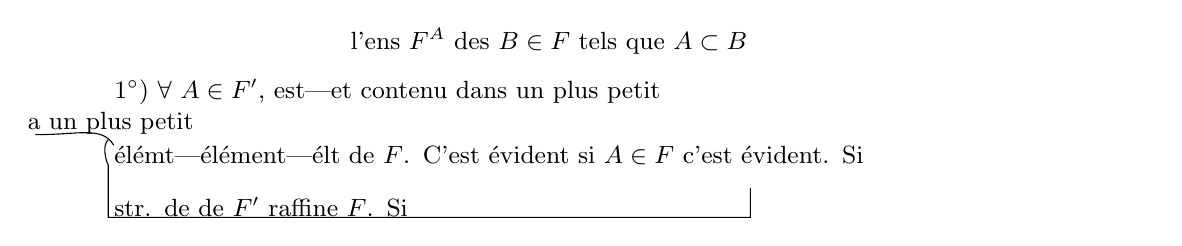
\begin{tikzpicture}[font=\small]
\node[anchor=north west,inner sep=0pt,text width=10.2cm] (family) at (3.0,0.65) {\deleted{\inserted{l'ens $F^A$ des $B\in F$ tels que $A\subset B$}}};
\node[anchor=north west,inner sep=0pt,text width=13.2cm] (attempt) at (0,0) {\deleted{1$^\circ$) \deleted{$\forall$} $A\in F'$, \unsure{est|et} \unsure{contenu dans} un plus petit}};
\node[anchor=north west,inner sep=0pt,text width=13.2cm] (resumption) at (0,-0.85) {\deleted{\unsure{élémt|élément|élt} de $F$. C'est évident si $A\in F$ c'est évident. Si}};
\node[anchor=north west,inner sep=0pt,text width=3.7cm] (addition) at (-1.1,-0.42) {\deleted{\inserted{\unsure{a un plus petit}}}};
\draw ([xshift=3pt]addition.south west) .. controls (-0.45,-0.72) and (-0.15,-0.6) .. (resumption.north west);
\node[anchor=north west,inner sep=0pt,text width=8cm] (abandoned) at (0,-1.5) {\deleted{\unsure{str.} de de $F'$ raffine $F$. Si}};
\draw ([xshift=-2pt,yshift=2pt]resumption.north west)
 .. controls (-0.15,-0.85) and (-0.10,-1.05) .. ([xshift=-2pt]resumption.south west)
 -- ([xshift=-2pt]abandoned.south west)
 -- ([xshift=2pt]abandoned.south east)
 -- ([xshift=2pt,yshift=3pt]abandoned.north east);
\end{tikzpicture}}

% @ lower part, restated first condition
1$^\circ$) \deleted{$\forall$} $A\in F'$, l'ens $F^A=\{B\in F\mid \deleted{B}A\subset B\}$ a un plus petit \unsure{élémt|élément|élt}. C'est évident si $A\in F$ \deleted{$(B=A)$} (on prend $B=A$) et si $A\in G'$, c'est vrai puisque $G'\ll F$.

% @ bottom, second condition
2$^\circ$) Si $A\in F'$, $B\in F$, alors $A\cap B$ est \deleted{\unsure{$\mathcal R_{F'}$-satu.|$\mathscr R_{F'}$-satu.}}\inserted{fermé dans $F'$}
% @ far right edge, beside the final replacement: two unlabelled curved pen strokes
\margin{\figure{\begin{tikzpicture}[x=1ex,y=1ex]
\draw (0,0.45) .. controls (0.25,0.95) and (0.9,1.1) .. (1,0.65)
 .. controls (0.82,0.15) and (0.30,0.12) .. (0.08,0.05);
\draw (0.25,0.45) .. controls (0.5,0.72) and (0.45,0.93) .. (0.7,0.98);
\end{tikzpicture}}}
, i.e. réunion de strates de $F'$. Si $A\in G'$, comme $G'\ll F$, $A\cap B$ est réunion de strates de $G'$, qui sont aussi des strates de $F'$.

\scanpage{32}\mspage{31}
% Adjudicated after the three independent readings and supplemental close checks.
% @ top, continuation
Si $A\in F\setminus G$, $A\cap B$ est réunion de strates de $F$. \deleted{Reste} reste \unsure{à|:} voir que une strate 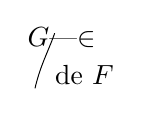
\begin{tikzpicture}[baseline=(de.base)]
\node[anchor=base west,inner sep=0pt] at (-.15,.48) {\inserted{\unsure{$G$|$\in$}}};
\node[anchor=base west,inner sep=0pt] (de) at (.2,0) {de $F$};
\draw[line width=.35pt] (-.05,-.05)..controls(.02,.25)and(.12,.42)..(.2,.65);
\end{tikzpicture} est réunion de strates de $F'$. Soit $A$ cette strate de $F$. \deleted{On}
\[
 \deleted{A=\bigcup_{\substack{B\in F\\B\leq F}}B^\circ}
\]
Si $A\notin G'$, alors $A\in F\mathbin{\underset{\begin{tikzpicture}[x=1ex,y=1ex,baseline=0pt]
\draw[line width=.45pt,line cap=round] (.30,.65) .. controls (.38,.36) and (.12,.18) .. (0,0);
\draw[line width=.45pt,line cap=round] (.16,.45)--(0,0)--(.20,0);
\end{tikzpicture}}{\setminus}}G'\subset F'$, et on gagne. Si $A\in G$, alors (comme $G'\preceq G$) $A$ est réunion de strates de $G'$, qui sont des strates de $F'$, et on gagne encore.

% @ left, oblique
\margin{Ultra faux}
% @ heading, subdivision and chacune interlinear
\figure{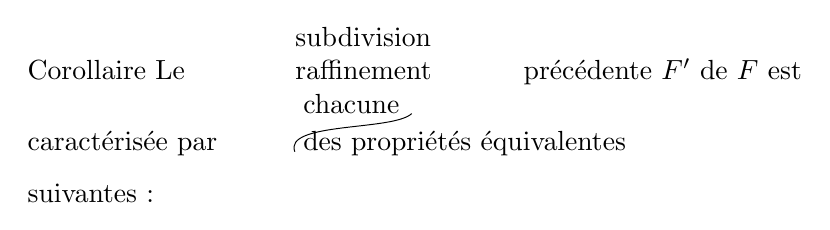
\begin{tikzpicture}[x=1cm,y=1cm]
\node[anchor=base west,inner sep=0pt] at (0,0) {\uline{Corollaire} Le};
\node[anchor=base west,inner sep=0pt] (oldnoun) at (3.4,0) {\deleted{raffinement}};
\node[anchor=base west,inner sep=0pt] at (3.4,.42) {\inserted{subdivision}};
\node[anchor=base west,inner sep=0pt] at (6.3,0) {précédente $F'$ de $F$ est};
\node[anchor=base west,inner sep=0pt] at (0,-.9) {caractérisée par};
\node[anchor=base west,inner sep=0pt] (chacune) at (3.5,-.42) {\inserted{chacune}};
\node[anchor=base west,inner sep=0pt] (des) at (3.5,-.9) {des propriétés équivalentes};
\draw[line width=.35pt] ([xshift=-.1cm,yshift=-.1cm]des.west)..controls(3.25,-.53)and(4.65,-.65)..([xshift=.15cm]chacune.south east);
\node[anchor=base west,inner sep=0pt] at (0,-1.55) {suivantes~:};
\end{tikzpicture}}

% @ whole a) crossed by two large diagonals; maximal also locally cancelled
\figure{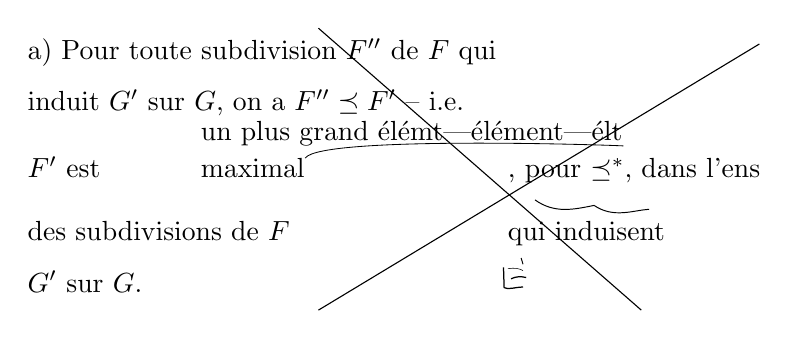
\begin{tikzpicture}
\node[anchor=base west,inner sep=0pt] at (0,0) {\deleted{a) Pour toute subdivision $F''$ de $F$ qui}};
\node[anchor=base west,inner sep=0pt] at (0,-.65) {\deleted{induit $G'$ sur $G$, on a $F''\preceq F'$ -- i.e.}};
\node[anchor=base west,inner sep=0pt] at (0,-1.5) {\deleted{$F'$ est}};
\node[anchor=base west,inner sep=0pt] (oldmax) at (2.2,-1.5) {\deleted{\uline{maximal}}};
\node[anchor=base west,inner sep=0pt] (newmax) at (2.2,-1.02) {\deleted{\inserted{un plus grand \unsure{élémt|élément|élt}}}};
\node[anchor=base west,inner sep=0pt] at (6.1,-1.5) {\deleted{, pour $\preceq^{*}$, dans l'ens}};
\draw[line width=.3pt] (oldmax.north east)..controls([xshift=.2cm,yshift=.3cm]oldmax.north east)and([xshift=.2cm]newmax.south east)..(newmax.south east);
\draw[line width=.35pt] (6.45,-1.78)..controls(6.7,-1.96)and(6.95,-1.9)..(7.2,-1.85)..controls(7.45,-2.02)and(7.7,-1.91)..(7.9,-1.9);
\node[anchor=base west,inner sep=0pt] at (0,-2.3) {\deleted{des subdivisions de $F$}};
\node[anchor=base west,inner sep=0pt] at (6.1,-2.3) {\deleted{qui induisent}};
\node[anchor=base west,inner sep=0pt] at (0,-2.95) {\deleted{$G'$ sur $G$.}};
% Unidentified angular mark directly below qui, inside the crossed block.
\begin{scope}[shift={(6.05,-2.91)},scale=.8]
\draw[line width=.45pt] (0,.34)--(.01,.02)..controls(.07,-.02)and(.20,.03)..(.31,.03);
\draw[line width=.45pt] (.12,.16)..controls(.21,.20)and(.27,.20)..(.36,.18);
\draw[line width=.2pt] (.07,.32)..controls(.18,.34)and(.26,.32)..(.31,.29);
\draw[line width=.35pt] (.28,.49)--(.31,.39);
\end{scope}
\draw[line width=.4pt] (3.7,.4)--(7.8,-3.18);
\draw[line width=.4pt] (3.7,-3.18)--(9.3,.2);
\end{tikzpicture}}
% @ oblique starred gloss
\margin{$*$ ou pour $\ll$, \unsure{cela|cel} revient au $=$ parmi des subdivisions d'une $=$ $F$}
% @ long oblique note, traversed by curved pen stroke
\margin{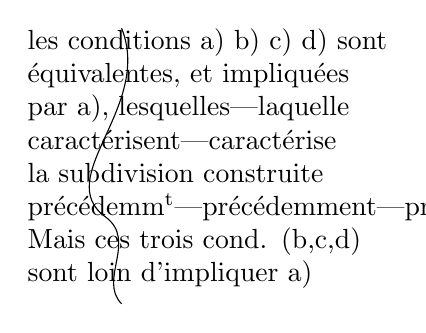
\begin{tikzpicture}
% The outer doubt concerns cancellation state, not the securely read words.
\node[anchor=north west,text width=4.7cm,inner sep=0pt] (note) at (0,0) {\unsure{\deleted{les conditions \deleted{\unsure{a)}} b) c) d) sont équivalentes, \unsure{et} \uline{impliquées} par a), \unsure{lesquelles|laquelle} \unsure{caractérisent|caractérise} la subdivision construite \unsure{précédemm\textsuperscript{t}|précédemment|précédemment\textsuperscript{\#}}. Mais ces trois \unsure{cond.} (b,c,d) sont \unsure{loin} d'impliquer a)}}};
\draw[line width=.4pt] ([xshift=1.2cm]note.north west)..controls(1.6,-1.0)and(.3,-1.9)..(1.0,-2.4)..controls(1.4,-2.7)and(.9,-3.2)..(1.2,-3.5);
\end{tikzpicture}}
b) L'application can. associée à $F'\preceq F$
\[
 \varphi:F'\longrightarrow F
\]
induit une bijection
\[
 F'\setminus G'\xrightarrow{\sim}F\setminus G.
\]
% @ right note, left vertical stroke
\margin{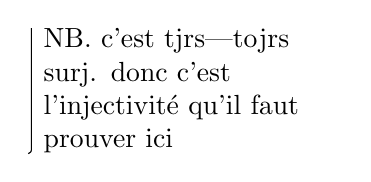
\begin{tikzpicture}
\node[anchor=north west,text width=3.8cm,inner sep=0pt] (nb) at (0,0) {NB. c'est \unsure{tjrs|tojrs} surj. donc c'est l'\uline{injectivité} qu'il faut prouver ici};
\draw[line width=.4pt] ([xshift=-.15cm]nb.north west)--([xshift=-.15cm,yshift=.08cm]nb.south west)..controls([xshift=-.15cm,yshift=.02cm]nb.south west)..([xshift=-.19cm]nb.south west);
\end{tikzpicture}}
% @ c): new sentence above the complete cancelled baseline, shared final de F'
c) \deleted{Les strates ouvertes de $F'$ qui ne sont} \inserted{$\forall A\in F\setminus G$, $A^\circ$ est une strate ouverte} de $F'$.
d) $F'\supset F\setminus G$, i.e. $\forall A\in F\setminus G$, on a $A\in F'$.
% @ foot: one On only
\uline{Dém} On va prouver p. ex
\[
 \text{d)}\Longrightarrow\text{b)}\Longrightarrow\text{c)}\Longrightarrow\text{a)}\Longrightarrow\text{d)}
\]
\deleted{\uline{Dém}} $\text{d)}\Rightarrow\text{b)}$ Si $(F\setminus G)\subset F'$, alors $\varphi\mid F\setminus G$ est l'\deleted{\unsure{identité}}\unsure{inclusion} \deleted{(trivial)} \inserted{can. $F\setminus G\hookrightarrow F$}, \deleted{donc} donc il reste à prouver
\[
 F\setminus G=F'\setminus G'.
\]

\scanpage{33}\mspage{32.}
% Adjudicated after three independent full readings and focused supplements.
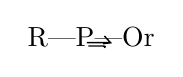
\begin{tikzpicture}[baseline=(old.base),x=1em,y=1em]
\node[inner sep=0pt] (old) at (0,0) {\deleted{\unsure{R|P|Or}}};
\draw[line width=.5pt] (-.15,-.2)--(.7,-.2)--(.48,.04);
\draw[line width=.5pt] (.7,-.2)--(.43,-.24);
\draw[line width=.5pt] (-.10,-.32)--(.40,-.32)..controls(.52,-.32)and(.54,-.35)..(.48,-.39);
\end{tikzpicture}
1°) $F\setminus G\subset F'\setminus G'$ i.e. Tout $A\in F\setminus G$ est $\notin G'$. En effet, si on avait $A\in G'$, on aurait $|A|\subset|G'|=|G|$ donc \deleted{$A\in$} (comme $G\leq F$) $A\in G$.

% @ vertical left margin, with long thin separation stroke
\margin{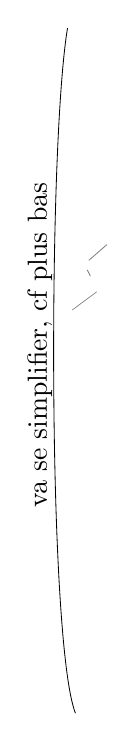
\begin{tikzpicture}
\node[rotate=90,anchor=west,inner sep=0pt] at (0,-1.8) {va se simplifier, cf plus bas};
\draw[line width=.3pt] (.35,4.3)..controls(.1,2.8)and(.1,-3.5)..(.45,-4.4);
% Two faint stroke clusters to the right of the rule, beside Je dis.
\draw[gray,line width=.3pt] (.62,1.35)--(.85,1.55);
\draw[gray,line width=.3pt] (.60,1.23)--(.64,1.15);
\draw[gray,line width=.25pt] (.41,.72)--(.72,.95);
\end{tikzpicture}}

2°) $F'\setminus G'\subset F\setminus G$ Soit $A'\in F'\setminus G'$, prouvons $A'\in F\setminus G$, et d'abord $A'\in F$. \deleted{On a} Soit $A$ le plus petit él. de $F^{A'}$ donc
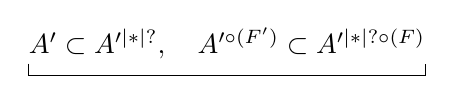
\begin{tikzpicture}[baseline=(f.base)]
\node[inner sep=0pt] (f) at (0,0) {$A'\subset A^{\deleted{\unsure{\prime|\ast|?}}},\quad A'^{\circ(F')}\subset A^{\deleted{\unsure{\prime|\ast|?}}\unsure{\circ(F)}}$};
\draw[line width=.4pt] ([yshift=-.05cm]f.south west)--([yshift=-.2cm]f.south west)--([yshift=-.2cm]f.south east)--([yshift=-.05cm]f.south east);
\end{tikzpicture}
prouvons que $A'\unsure{\deleted{\unsure{\in|\subset}}=|\in}A$ (d'où $A\in F$). \deleted{On a}

Je dis que $A\in F\setminus G$ i.e. $A\notin G$, sinon on aurait $A\subset|G|=|G'|$ donc $A'\in G'$ puisque $A'\in F'$ et $G'\leq F'$, absurde. \deleted{Mais} Donc $A\in F\setminus G$, donc $A\in F'$, \deleted{et} Il en résulte que $A^{\circ(F)}=A^{\circ(F')}$
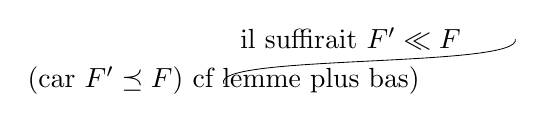
\begin{tikzpicture}[baseline=(lemma.base)]
\node[anchor=base west,inner sep=0pt] (lemma) at (0,0) {(car $F'\preceq F$\deleted{)} cf lemme plus bas)};
\node[anchor=base west,inner sep=0pt] at (2.7,.5) {\inserted{il suffirait $F'\ll F$}};
\draw[line width=.3pt] (2.5,.05)..controls(2.3,.43)and(6.3,.25)..(6.2,.62);
\end{tikzpicture}
et \unsure{\uline{bien}|\deleted{bien}} \deleted{$\unsure{F|\in|\exists}$} $A,A'\in F'$ tels que $A'^{\circ(F')}\subset A^{\circ(F')}$, ce qui prouve $A=A'$.

Donc \unsure{on a} prouvé que $\deleted{\unsure{F|A}}A'\in F'\setminus G'\Rightarrow A'\in F$. Prouvons qu'on a $A'\notin G$ (d'où $A'\in F\setminus G$\deleted{)}, qed). Sinon on aurait $A'\in G$, on aurait $A'\subset |G|=|G'|$, d'où
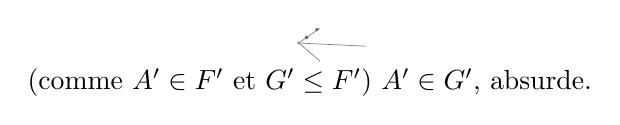
\begin{tikzpicture}[baseline=(last.base)]
\node[anchor=base west,inner sep=0pt] (last) at (0,0) {(comme $A'\in F'$ et $G'\leq F'$) $A'\in G'$, absurde.};
% Separate pale mark above et: reproduced without assigning a mathematical role.
\draw[gray,line width=.25pt] (4.3,.55)--(3.45,.59)--(3.72,.78);
\draw[gray,line width=.25pt] (3.45,.59)--(3.72,.36);
\fill[black!60] (3.55,.66) circle (.025);
\fill[black!60] (3.68,.76) circle (.025);
\fill[black!45] (3.45,.59) circle (.02);
\end{tikzpicture}

% @ abandoned argument, with upper insertion and five oblique strokes
\figure{\begin{tikzpicture}
\node[anchor=base west,inner sep=0pt] at (2.8,.55) {\deleted{\inserted{On suppose b) i.e. $\varphi$ induit $F'\setminus G'\overset{\sim}{\longrightarrow}F\setminus G$}}};
\node[anchor=base west,inner sep=0pt] at (0,0) {\deleted{b) $\Rightarrow$ c) Soit $A\in F\setminus G$, prouvons que}};
\node[anchor=base west,inner sep=0pt] at (0,-.75) {\deleted{$A^{\circ(F)}$ est une \uline{strate ouverte \deleted{dans \unsure{la}} de} $F'$. Soit}};
\node[anchor=base west,inner sep=0pt] at (0,-1.5) {\deleted{$A'\in F'\setminus G'$ l'unique élément \deleted{de} tel que $\varphi(A')=A$.}};
% The final uncrossed baseline may share the paragraph-level cancellation.
\node[anchor=base west,inner sep=0pt] at (0,-2.25) {\unsure{\deleted{Prouvons $A'^{\circ(F')}=A^{\circ(F)}$.}}};
\draw[line width=.3pt] (2.65,-.2)..controls(2.4,.35)and(11.7,.2)..(11.9,.62);
\draw[line width=.4pt] (.15,-1.7)--(1.65,.45);
\draw[line width=.4pt] (2.5,-1.8)--(4.2,.55);
\draw[line width=.4pt] (5.4,-1.7)--(7.1,.6);
\draw[line width=.4pt] (8.1,-1.65)--(9.7,.55);
\draw[line width=.4pt] (10.4,-1.65)--(11.7,.4);
\end{tikzpicture}}

b $\Longleftrightarrow$ c \deleted{Posons} On a $|F|\setminus|G|=|F'|\setminus|G'|$, soit $U$, Posons $F\setminus G=I^{\unsure{k|\ast|+}},\ F'\deleted{\unsure{\times|\setminus}}\unsure{\setminus}G'=I'^{\unsure{k|\ast|+}}$ (parties ouvertes des ens d'indices ordonnés $\unsure{I|\vec I}$, \deleted{$\unsure{A|\Delta}$} $(=F)$, $I'(=F')$. On a
